\documentclass[CS5104-Notes.tex]{subfiles}
\begin{document}

\section{Linear regression}
Linear regression models are simple but can provide a good and adequate descriptions of how the inputs affect the output. As linear regression only deals with linear models, it follows from the linear line equation $y = mx + c$ where the gradient $m$ and intercept $c$ are the $\theta$ parameters that the model tries to learn. This can be rewritten as:
\begin{equation}
f(X, \theta) = \theta_{0} + \theta_{1}X_{1}
\end{equation}
where $\theta_{0}$ represents the $c$ intercept and $\theta_{1}$ represents the $m$ gradient.
\n
Furthermore, a loss function has to be defined to evaluate the quality of the fit without manual inspection. The goal of training is to reduce the error of the loss function. This is done by trying lots of different $\theta$ values and computing the error each time. 

\subsection{Gradient descent}
Gradient descent is a method for parameter optimisation which automatically gets to the best model by minimising the lost function and automatically altering the $\theta$ parameters.
\begin{equation}
  \theta_{j} := \theta_{j} - \alpha \frac{\delta}{\delta \theta_{j}} L(\theta_{0}, \theta_{1})
\end{equation}
where j = 0 and j = 1 update is done simultaneously. $\alpha$ here is the learning rate, which acts as a modifier to how much should be updated on each iteration. $\frac{\delta}{\delta \theta_{j}} L(\theta_{0}, \theta_{1})$ is the derivative. The derivative of the loss function is used to see if we should increase or decrease the value of $\theta$.
\begin{figure}[H]
  \centering
  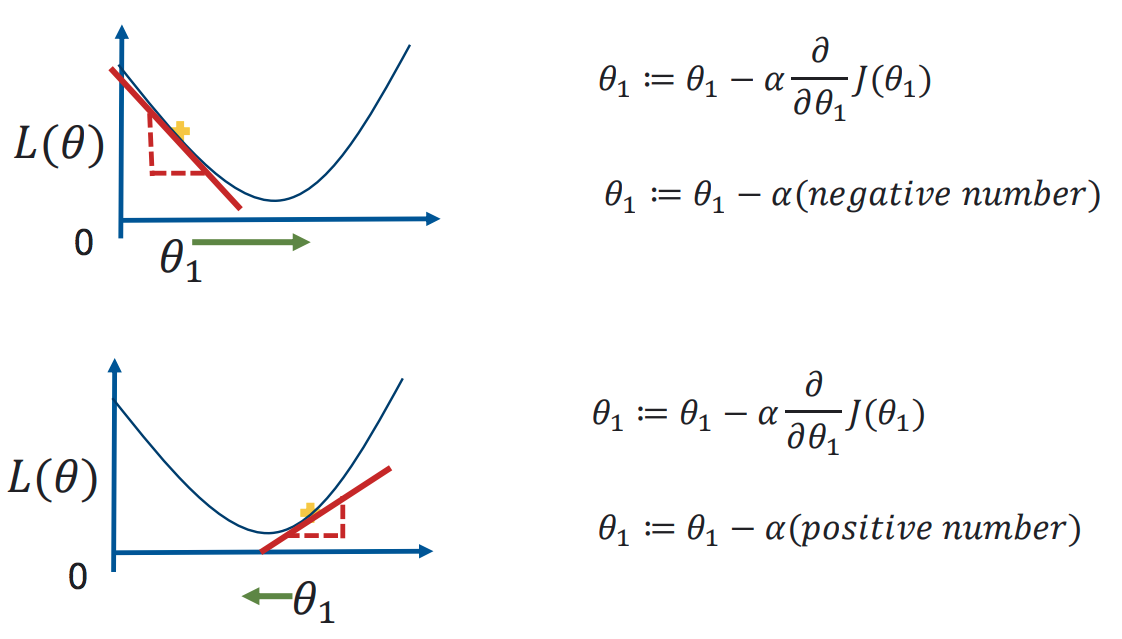
\includegraphics[width=0.9\textwidth, keepaspectratio]{imgs/gradient-descent.png}
  \caption{Gradient descent updating based on positive or negative gradient. For example, if the gradient is negative, we want to increase the $\theta$ values and recalculate the gradient.}
\end{figure}
There is an issue with gradient descent where it can get stuck in an local minimumm rather than the global minimum. There are a few ways of dealing with this:
\begin{itemize}
\item Try different initial values to start at different locations in the search space
\item Add momentum to roll over local minima
\end{itemize}
A good way to find out what is happening with each training iteration is to plot the cost function at each iteration, then it can be seen if the cost is being minimised. The reduction of the cost function is controlled by the \textbf{learning rate} $\alpha$. If $\alpha$ is too small, the gradient descent will be slow, requiring a large number of training iterations to minimise the cost and converge at the minimum. However, if the learning rate is too high, then it can overshoot the minimum and never converge. This effect can be seen by plotting the cost function and seeing if the graph converges to 0 or diverges. 

\subsection{Multivariate linear regression}
Linear models can have many features and by extending to $n$ features with $n$ $\theta$ parameters. This extends the linear equation to be:
\begin{equation}
f(x) = \theta_{0} + \theta_{1}x_{1} + \theta_{2}x_{2} + ... \theta_{n}x_{n}
\end{equation}
The input features $X$ and parameters $\theta$ can be more easily represented with matrix form:
\begin{equation}
X = \begin{bmatrix}
X_{0} \\
X_{1} \\
X_{2} \\
\vdots \\
X_{n}
\end{bmatrix}
\end{equation}
Using matrix operations, all $\theta$ parameters can be updated simultaneously on every step rather than separately.

\subsection{Feature scaling}
When there are many input features, they can come from different scales. For example, one feature may have the range 0-1 while another has values ranging from 100-1000. Because of these different scales, the larger values may dominate the model even if both features are equally important. To deal with this issues, all features can be scaled to the same range through normalisation.
\begin{equation}
x_{i} = \frac{x_{i} - \mu_{i}}{\text{range}(x_{i})}
\end{equation}
One method of feature scaling is mean normalisation, where each input feature $x_{i}$ is replaced with $x_{i} - \mu_{i}$ to make features with a mean of approximately zero. 

\subsection{Normal equation}
\begin{equation}
\theta = (X^{T}X)^{-1}X^{T}y
\end{equation}
where $X^{T}$ is the transpose of X and $(X^{T}X)^{-1}$ is the inverse of $X^{T}X$. Feature scaling is not needed for the normal equation because each $\theta$ parameter is proportional to the input feature it is calculated from. $X$ and $y$ here are matrices of the inputs and outputs. With the normal equation, the $\theta$ parameters can be calculated analytically rather than require the many training iterations. It is sometimes preferable to use the normal equation over optimisation like gradient descent as there is not need for computation iterations and choice of learning rate. However, the normal equation is slow to calculate if the number of input features is very large, which gradient descent deals with well. 


\begin{minipage}{0.45\textwidth}
\textbf{Normal equation} \n
Pros:
\begin{itemize}
\item No need for iteration
\item Don't need to choose $\alpha$
\end{itemize}
Cons:
\begin{itemize}
\item Slow if number of input features is very large
\end{itemize}
\end{minipage}
\hspace*{\fill}
\begin{minipage}{0.45\textwidth}
\textbf{Gradient descent} \n
Cons:
\begin{itemize}
\item Needs many iterations
\item Need to choose learning rate $\alpha$
\end{itemize}
Pros:
\begin{itemize}
\item Works well when the number of features is large
\end{itemize}
\end{minipage}

\section{Logistic regression}
Logistic regression is a machine learning model to classify input data into output classes. A typical example of using logistic regression is to classify cancer or not cancer. We cannot use linear regression for classification tasks as it does not fit the data well and therefore is not well suited. In classification, a \textbf{sigmoid function} is used as it gives values between 0 and 1, like a switch between binary values. Coincidentally, sigmoid functions are also used as activation functions in neural networks. 
\n
The sigmoid function is defined as follows:
\begin{equation}
g(z) = \frac{1}{1 + e^{-z}}
\end{equation}
where $z = \theta^{T}x$. With classification, the output is typically a probability that of a certain class $ 0 \leq h(x) \leq 1$. The function is therefore:
\begin{equation}
h(x) = g(\theta^{T}x) = \frac{1}{1 + e^{-\theta^{T}x}}
\end{equation}
where $h(x)$ is the estimated probability that $y = 1$ on input $x$. In an example of multiple input features, we get get multiple $\theta$ values. For example, given blood and urine test values, does the patient have cancer:
\begin{equation}
h(x) = g(\theta^{T}x) = g(\theta_{0} + \theta_{1}x_{1} + \theta_{2}x_{2}) =  \frac{1}{1 + e^{-\theta^{T}x}}
\end{equation}
where $x_{1}$ is the blood test values and $x_{2}$ is the urine test values. $h(x)$ is the probability that the patient has cancer.
\begin{figure}[H]
\centering
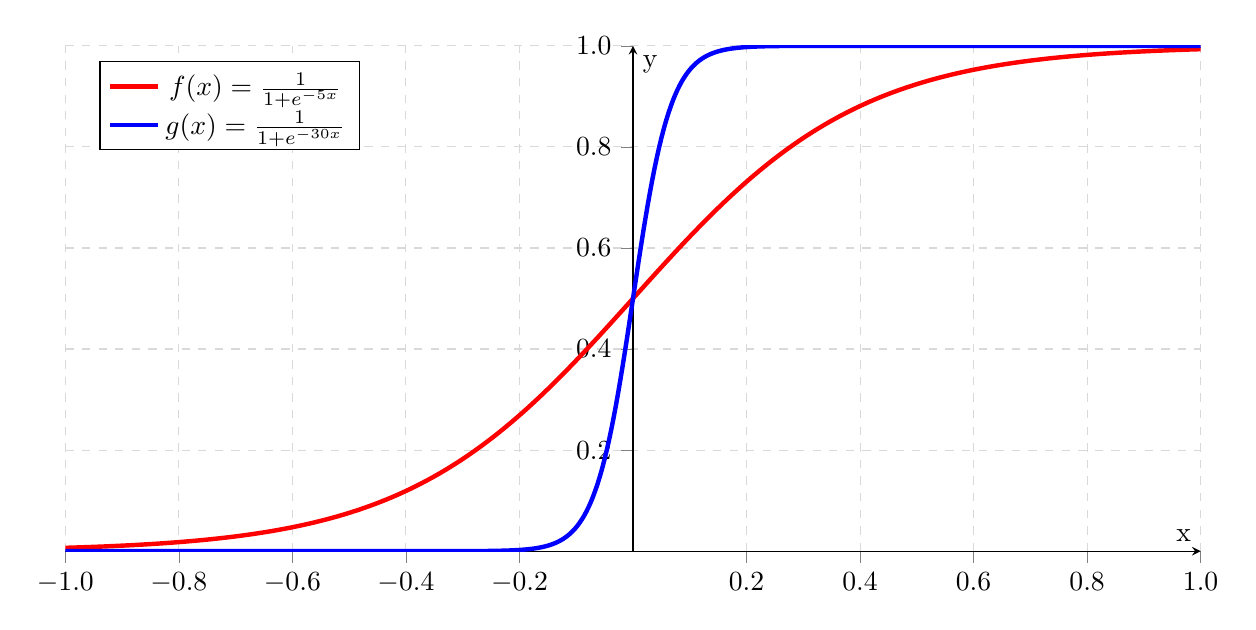
\begin{tikzpicture}
    \begin{axis}[
    	legend pos=north west,
        axis x line=middle,
        axis y line=middle,
        x tick label style={/pgf/number format/fixed,
                            /pgf/number format/fixed zerofill,
                            /pgf/number format/precision=1},
        y tick label style={/pgf/number format/fixed,
                            /pgf/number format/fixed zerofill,
                            /pgf/number format/precision=1},
        grid = major,
        width=16cm,
        height=8cm,
        grid style={dashed, gray!30},
        xmin=-1,     % start the diagram at this x-coordinate
        xmax= 1,    % end   the diagram at this x-coordinate
        ymin= 0,     % start the diagram at this y-coordinate
        ymax= 1,   % end   the diagram at this y-coordinate
        %axis background/.style={fill=white},
        xlabel=x,
        ylabel=y,
        tick align=outside,
        enlargelimits=false]
      % plot the stirling-formulae
      \addplot[domain=-1:1, red, ultra thick,samples=500] {1/(1+exp(-5*x))};
      \addplot[domain=-1:1, blue, ultra thick,samples=500] {1/(1+exp(-30*x))};
      \addlegendentry{$f(x)=\frac{1}{1+e^{-5x}}$}
      \addlegendentry{$g(x)=\frac{1}{1+e^{-30x}}$}
    \end{axis}
\end{tikzpicture}
\caption{Example of a sigmoid function. The parameters $\theta^{T}$ determine the steepness.}
\end{figure}
\noindent
For some classification problems, a linear logistic regression model is not enough. This happens when a linear decision boundary is not enough to distinguish between the different classes. In these cases, a non-linear function is needed.

\subsection{Cost function}
In logistic regression, the same squared error cost used in linear regression cannot be used because it doesn't make much sense. A cost function such as the squared error measures the \textit{distance} between the predict value and actual value, however, this distance is not easily identified for a classification problem, where the actual value is which class the data belongs in. 
\begin{align}
Cost(h(x),y) &= \begin{cases}
	-log(h(x)) & \text{if } y = 1 \\
	-log(1-h(x)) & \text{if } y = 0
      \end{cases} \\
Cost(h(x),y) &= -ylog(h(x)) - (1 - y)log(1 - h(x))
\end{align}
\begin{figure}[H]
\centering
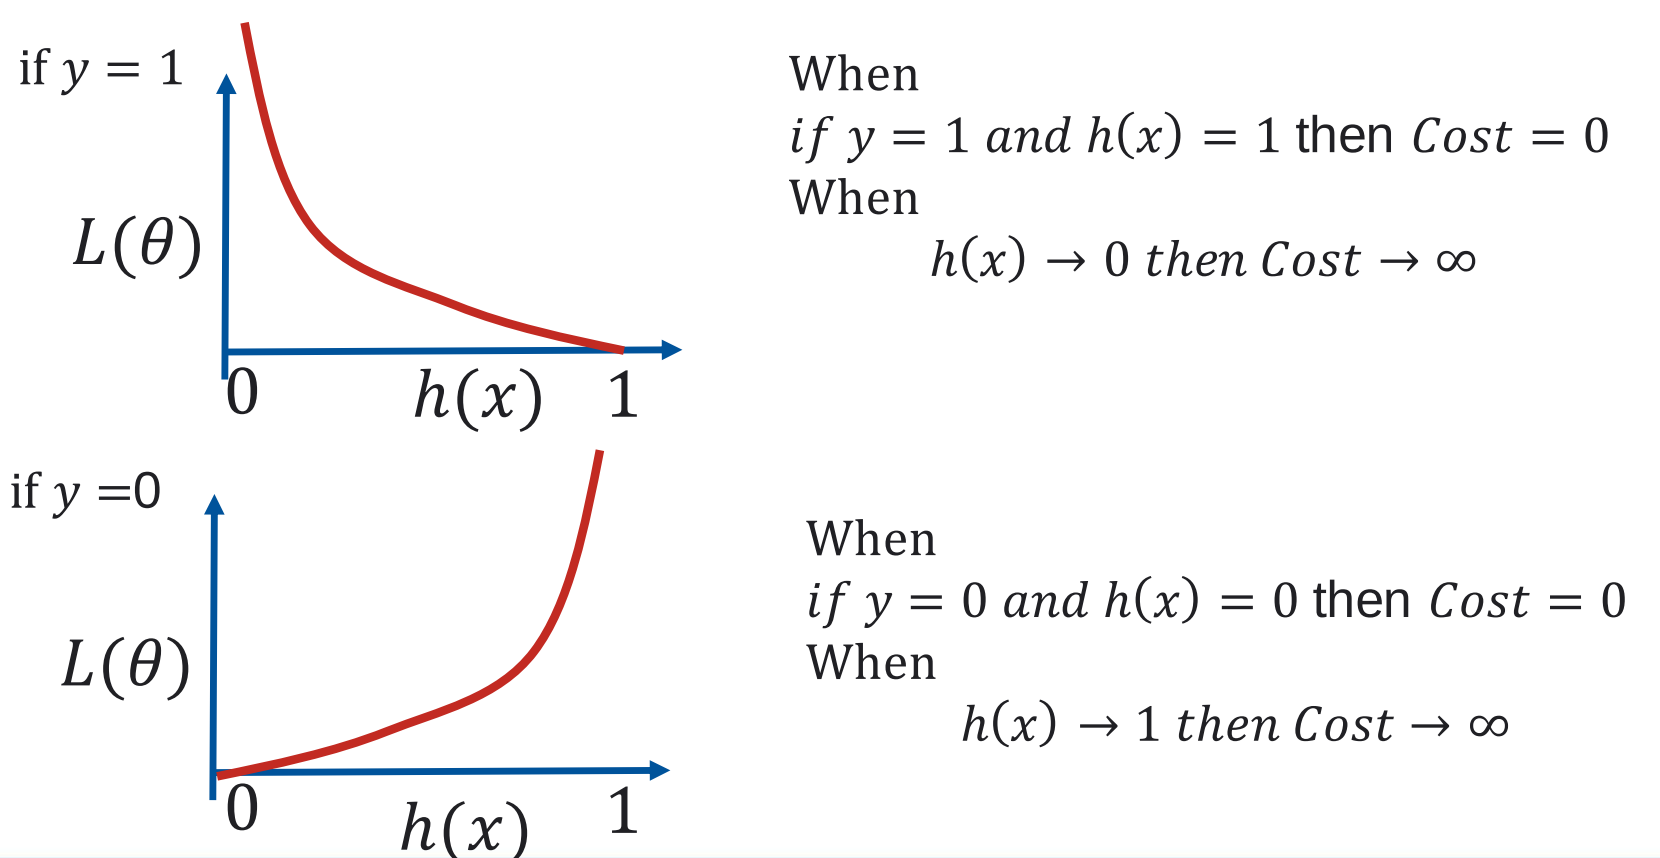
\includegraphics[width=0.9\textwidth, keepaspectratio]{imgs/logistic-regression-cost.png}
\caption{Cost function for logistic regression.}
\end{figure}
\noindent
Log functions are used as the cost function so that the cost for a prediction of $h(x) \approx 1$ tends to 0 and a prediction of $h(x) \approx 0$ tends to $\infty$. This this cost function, logistic regression can also use gradient descent to tweak $\theta$ parameters.

\subsection{Multiclass classification}
There are often cases in classification where it is not simply a binary classification such as cancer or not cancer. This is multiclass classification where there are multiple classes, such as classifying the colour based on wavelength. Here, simply applying the previous techniques and cost functions is not enough as it will only give the probability of one certain class. To deal with multiclass problems, the typical solution is to use a \textbf{one-vs-all} method where each class is treated separately as a binary classification task. There are three main steps for doing this:
\begin{itemize}
\item Choose one class apply binary classification to all data points
\item Repeat for all other classes
\item Generate probability for each class based on the binary classification and pick the classification with the highest probability
\end{itemize}


\end{document}